\label{detbeamtest}
One of the main goals of the Single-Phase Prototype test beam program is to perform measurements 
needed to control and understand systematic uncertainties in DUNE oscillation measurements.
The program also includes measurements to support other important DUNE physics measurements as described below.
%detector is intended to provide input necessary to reduce systematic uncertainties for oscillation measurements 
%

%Current assumptions on detector related systematic uncertainties in DUNE to achieve
%projected sensitivities~\cite{DuneCDR} are shown in
%%Assumptions on current level of uncertainties are shown in 
%Table \ref{table:deterr}. These are compared with teh levels achieved in MINOS and T2K
%appearance measurements.
%\begin{table}[h]
%\centering
%\caption{Current estimated detector related  sources of uncertainty for oscillation 
%measurements.}
%\label{table:deterr}
%\begin{tabular}{|l|c|c|c|l|}
%\hline
%\textbf{Source of uncertainty } & \textbf{MINOS} & \textbf{T2K} & \textbf{DUNE} & \textbf{Comments}  \\ \hline
%$\nu_e$ energy scale  & 2.7\% & 2.5\% & 2\% & comment \\ \hline
%\end{tabular}
%\end{table}
%% THIS IS FROM TABLE 3.8 of CDR


As an example of the importance of controlling detector related uncertainties,
Fig.~\ref{fig:spectraleffect} shows the effect of a lepton energy scale 
uncertainty of -5\% on the measured 
appearance signal (for $\delta_{CP}=0$) and backgrounds in DUNE. 
The crosses shows the expected signal shape for $\delta_{CP}=+\pi/2$ and -$\pi/2$. 
Energy scale uncertainties can mimic a non-zero
$\delta_{CP}$ phase. 
\begin{figure}[h!]
\centering
%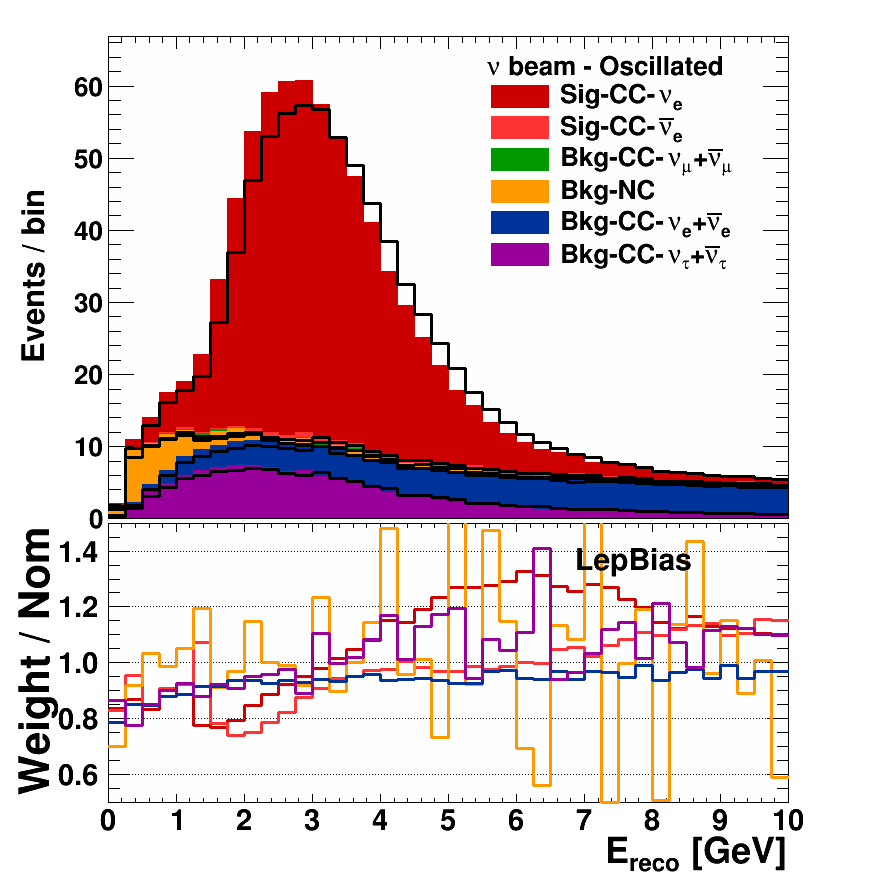
\includegraphics[width=0.7\textwidth,height=7.7cm]{figures/lepbias10}
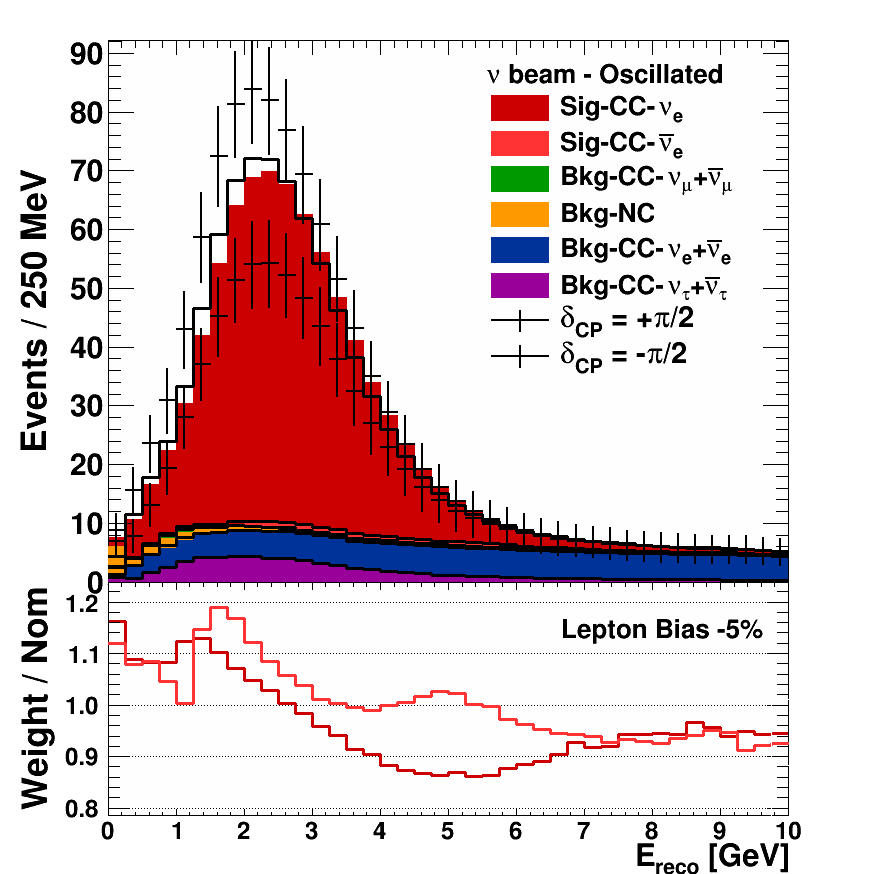
\includegraphics[width=0.7\textwidth,height=7.7cm]{figures/CSPP_LeptonBias_nue_app_FHC}
\label{fig:spectraleffect}
  \caption{DUNE $\nu_e$ appearance signal and background spectra assuming 
$\delta_{CP}=0$. 
Solid curves shows the effect of -5\% lepton energy scale shift on the 
measured appearance signal 
and backgrounds. 
The crosses shows the expected signal shape for $\delta_{CP}=+\pi/2$ and -$\pi/2$. 
Ratios show the distortion on the $\nu_e$ and $\overline{\nu}_e$ spectra due to the 
5\% energy scale shift. 
}
\end{figure}
Effects on sensitivity to mass hierarchy and $\delta_{CP}$ as a function of 
$\delta_{CP}$ are shown in Fig.~\ref{fig:global_escale_sens} from Ref.~\cite{dunecdr}. 
%shows the effect of various levels of neutrino energy on sensitivities. 
The nominal sensitivity assumes a 230-kt-MW-year 
exposure with equal neutrino and antineutrino mode running. 
This does not account for correlated uncertainties in neutrino and 
antineutrino running or effects on backgrounds and is therefore likely
a best-case scenario. 
\begin{figure}[h!]
\centering
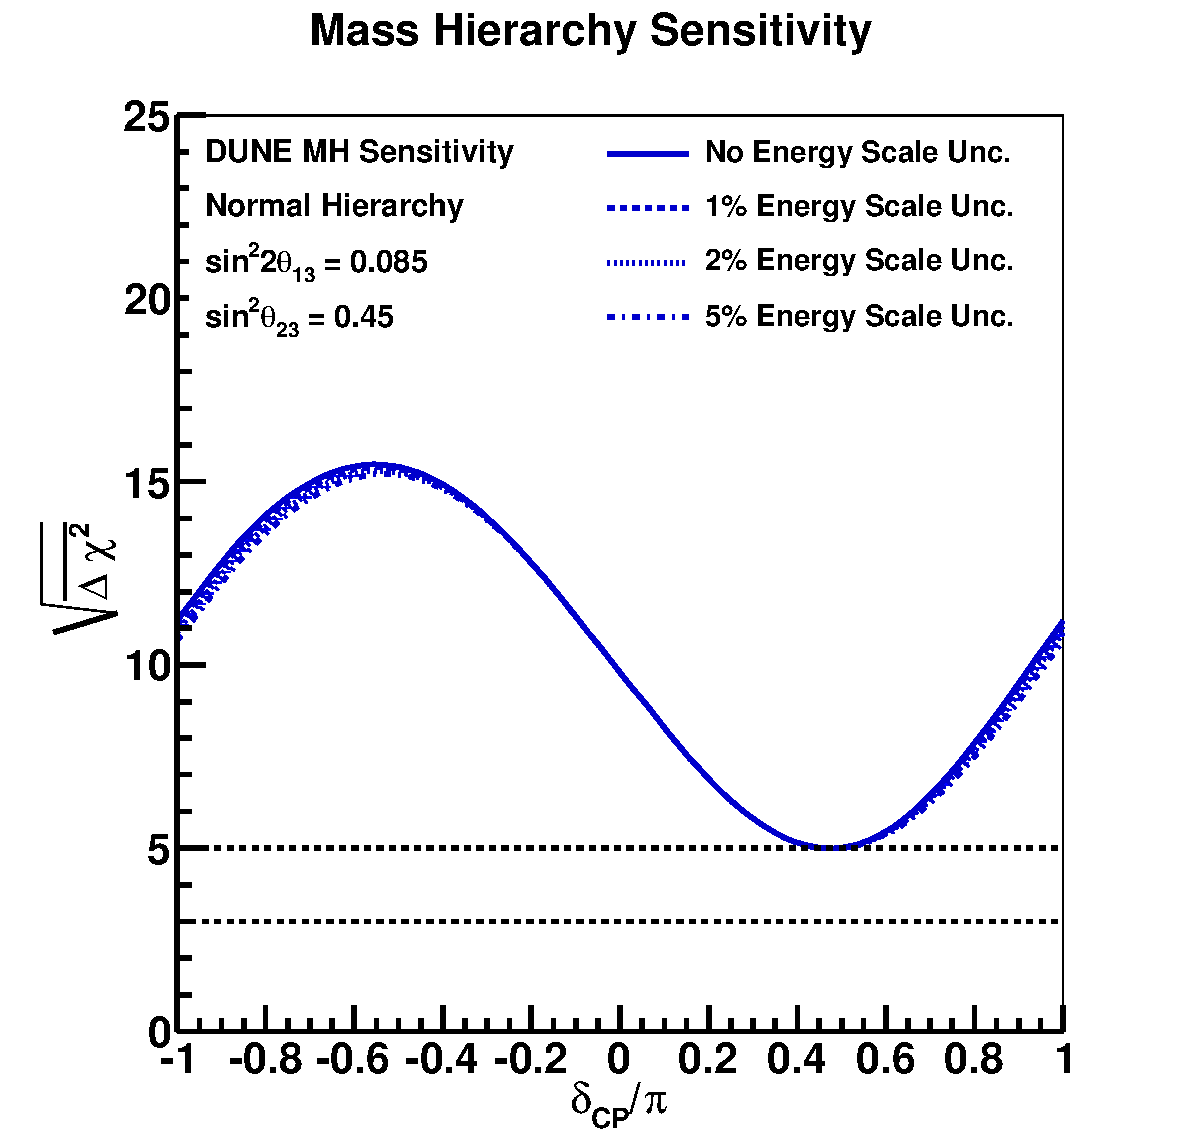
\includegraphics[width=0.49\textwidth,height=6.7cm]{figures/mh_230ktmwyear_varyesyst}
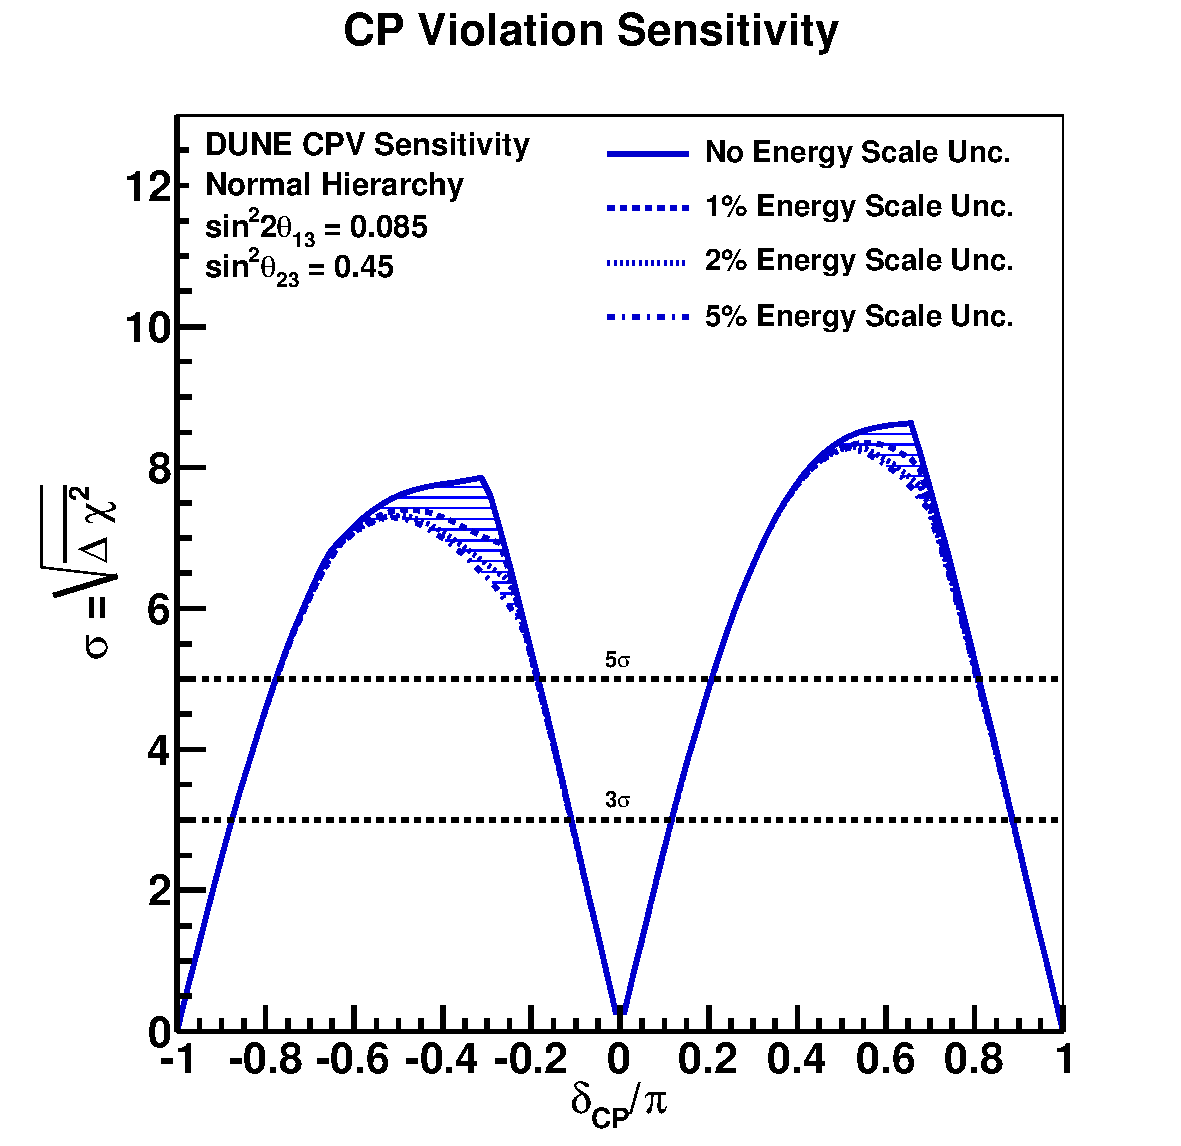
\includegraphics[width=0.49\textwidth,height=6.7cm]{figures/cpv_890ktmwyear_varyesyst}
%\includegraphics[width=0.49\textwidth,height=6.7cm]{figures/mh_escale_sens}
%\includegraphics[width=0.49\textwidth,height=6.7cm]{figures/deltacp_escale_sens}
\label{fig:global_escale_sens}
  \caption{DUNE projected sensitivity dependence of mass hierarchy (left) and $\delta_{CP}$ 
(right) to neutrino energy scale uncertainties. 
If energy scale uncertainties can be controlled at the appropriate levels, DUNE can achieve 
at least 5$\sigma$ sensitivity on mass hierarchy determination for 100\% of $\delta_{CP}$ values and
for 3$\sigma$ sensitivity to  $\delta_{CP}$ for 75\% coverage of phase space.
{\color{red} 
Need to check details of assumptions
}
}
\end{figure}

Work to evaluate effect of all systematic uncertainties in DUNE sensitivities is still in progress. Current levels of sensitivity in ~\cite{dunecdr} assumes
$\nu_e$ energy scale is known at the level of 2\%. 
More here...
%will require a dedicated test beam


%$\nu_e$ energy scale  & 2.7\% & 2.5\% & 2\% & comment \\ \hline
%\end{tabular}


\subsection{Summary of Detector and Beam Requirements }
\label{detbeam_main}

LAr TPC technology was first proposed for use in neutrino experiments by C. Rubbia in 1977
\cite{Rubbia} but extensive use in neutrino experiments is only now being realized. 
%CERN-EP-INT-77-8
%Title 	The liquid-argon time projection chamber : a new concept for neutrino detectors
%operating in the CNGS beamline  (with mean beam energy $\sim$17 GeV)~\cite{ICARUSmain}. 
The ICARUS T600 detector~\cite{icarus_mainref} pioneered the first large-scale detector operating in the CNGS 
neutrino beam at mean energy $\sim$17 GeV. ArgoNeuT~\cite{argoneut1}\cite{argoneut2} recently studied 
neutrino interactions in the NuMI beam down to sub-GeV energies with a small-scale (170~$l$ fiducial volume) detector. 
While these samples are proving useful, they do now allow full isolation of
the low energy neutrino interaction processes
and final states from reconstruction and detector effects. 
The use of this technology in future precision neutrino experiments will require dedicated 
information on particle response
in the few-GeV to sub-GeV range provided by charged-particle test beams. 

%%%
%\subsubsection{Particles energy and direction}
%\label{detbeam_particles}
The DUNE experiment will run beam in both neutrino and anti-neutrino 
configurations. These beams will be composed  mainly of muon neutrinos (anti-neutrinos) as well as electron neutrinos (anti-neutrinos). In Fig. \ref{fig:particle_momenta} the distributions of momenta and angles of particles created in neutrino interactions from simulated beam fluxes are shown. The rate on the particles are calculated for the 34kton far detector and  are combined from both neutrino and anti-neutrino beams. In addition the electron rates from charged current interactions for muon neutrinos oscillated to electron neutrinos are shown. 
\begin{figure}[h!]
  \centering
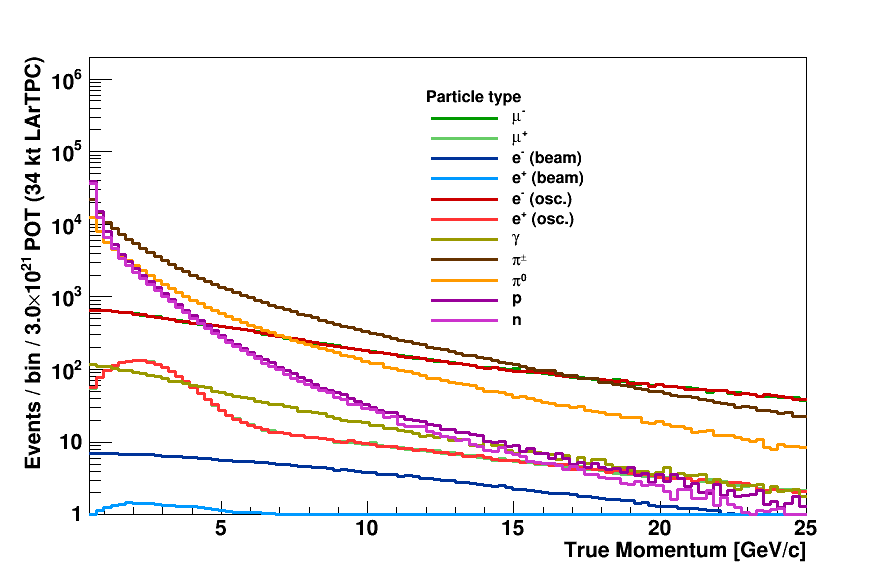
\includegraphics[width=0.49\textwidth,height=5.0cm]{figures/True_Momenta_per_Particle_9_2_1_0_log}
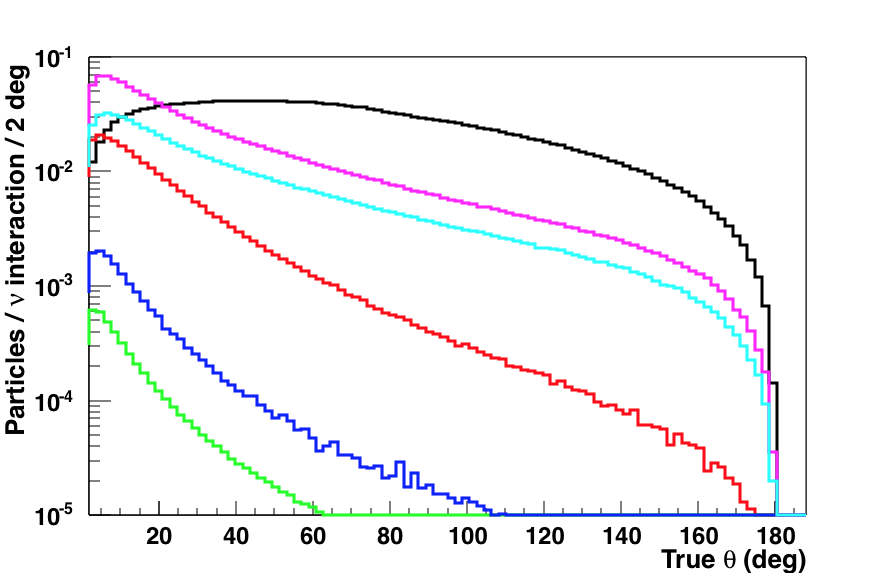
\includegraphics[width=0.49\textwidth,height=5.0cm]{figures/True_theta_per_Particle_9_2_1_0_lin}
  \caption{Particle momenta (left) and angular (right) distributions for particles produced in neutrino interactions 
from $\nu_e$, $\nu_\mu$, $\bar \nu_e$ and $\bar \nu_\mu$ at the far detector location.
{\color{red}  combine e+e-, improve information content (y-axis, change colors, etc )
}
}
\label{fig:particle_momenta}
\end{figure}


%\begin{figure}[h!]
%  \centering
%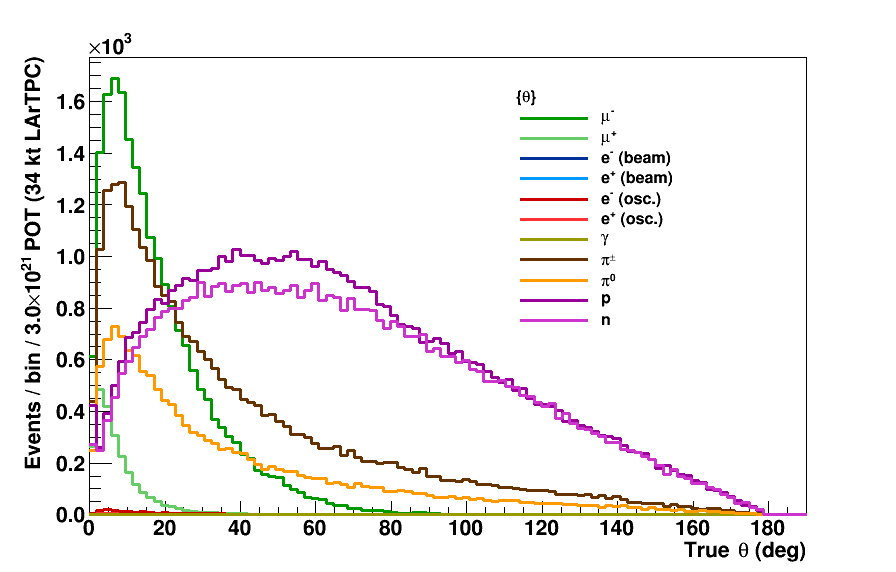
\includegraphics[scale=0.4]{figures/True_theta_per_Particle}
%\label{fig:particle_theta}
%  \caption{Particle angle wrt to the beam axis distributions for particles coming from all fluxes ($\nu_e$, $\nu_\mu$, $\bar \nu_e$ and $\bar \nu_\mu$) at both near and far detector locations.  }
%\end{figure}

%\newpage

The detector is designed from components that match exactly the current DUNE far detector design components. 
The test beam detector must be sufficiently large in both
longitudinal and transverse dimensions to contain showering particles up to the energy range of interest ($\sim$10~GeV).
Fig.~\ref{fig:containment} shows the simulated longitudinal and transverse 
energy containment for proton showers up to 10~GeV in energy.
For 10 GeV showers, more than 95\% of the energy is contained in a detector of longitudinal size of 6~m and 
radius of 2.5~m. Shower from pions, kaons, and electrons have also been studied and better containment
is achieved in those cases. 
\begin{figure}[htp]
  \centering
  \begin{tabular}{ccc}
%    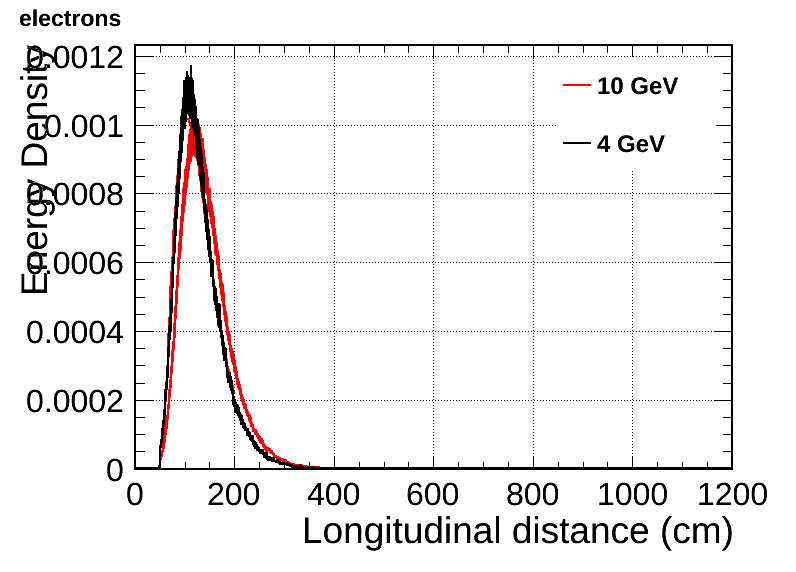
\includegraphics[scale=0.15]{figures/electrons_density_overlay}&
%    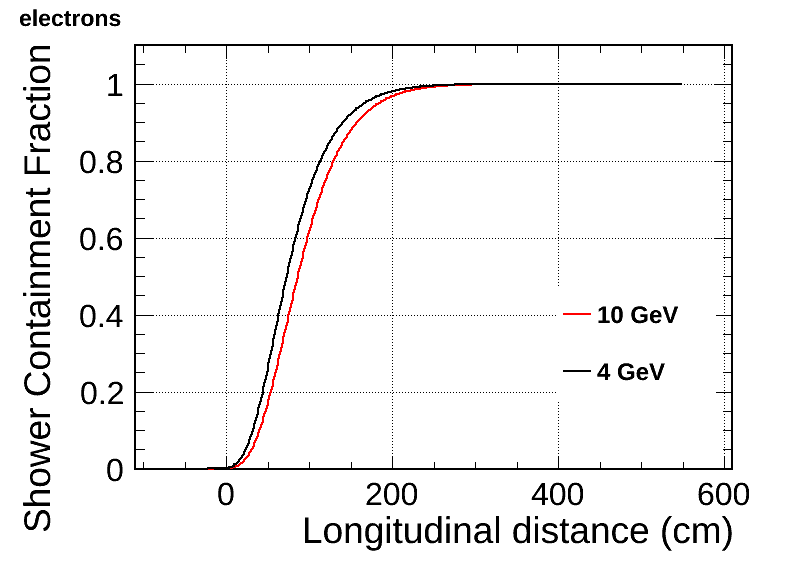
\includegraphics[scale=0.15]{figures/electrons_lcont_overlay}&
%    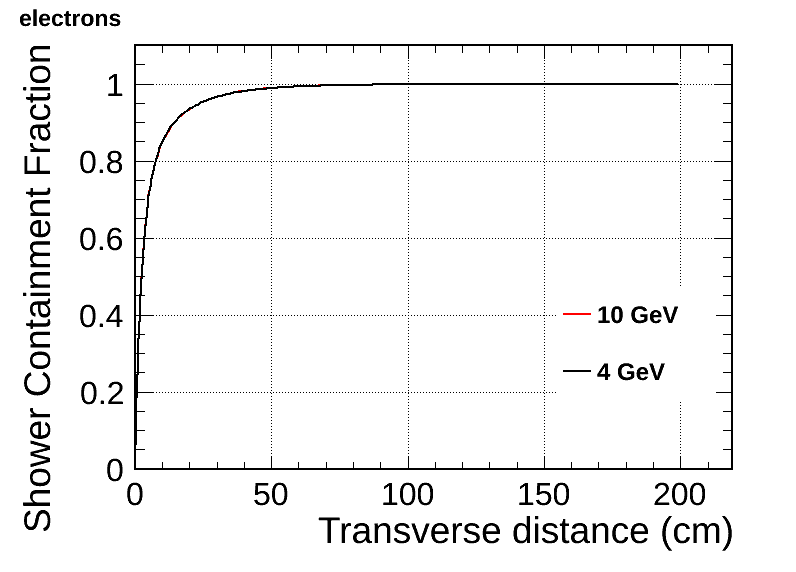
\includegraphics[scale=0.15]{figures/electrons_wcont_overlay}\\
%  
%    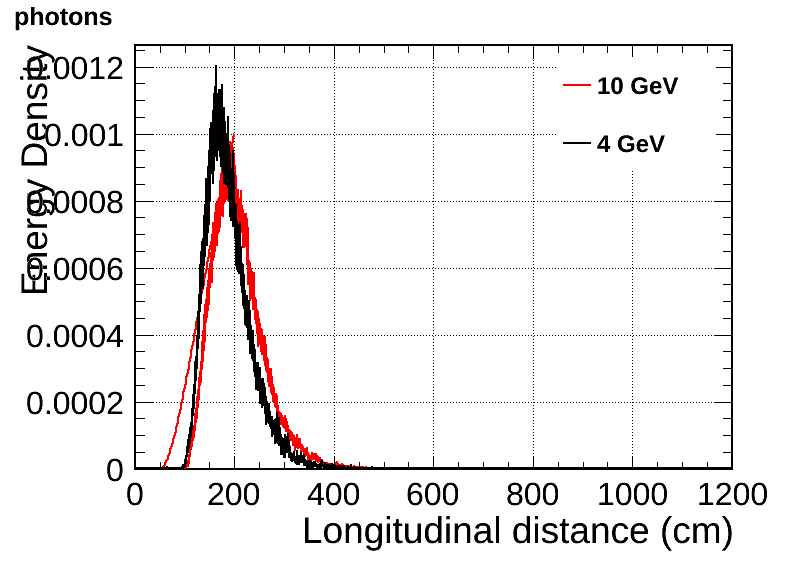
\includegraphics[scale=0.15]{figures/photons_density_overlay}&
%    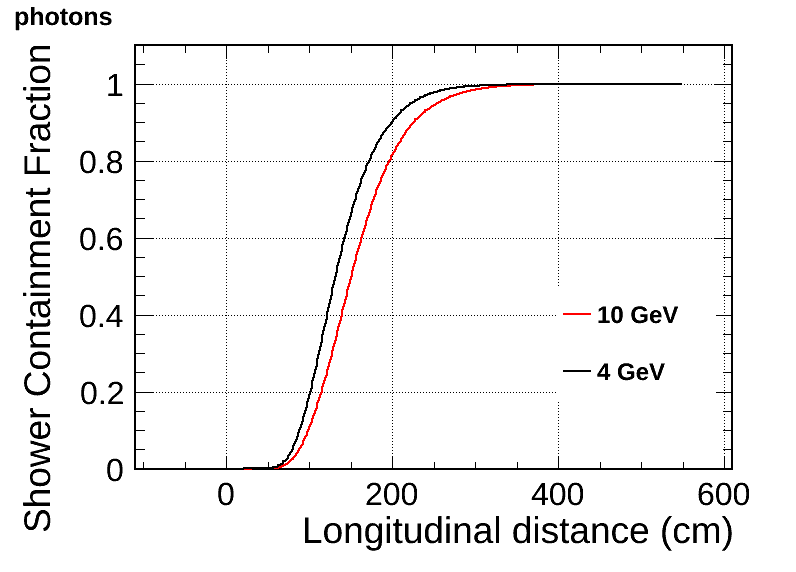
\includegraphics[scale=0.15]{figures/photons_lcont_overlay}&
%    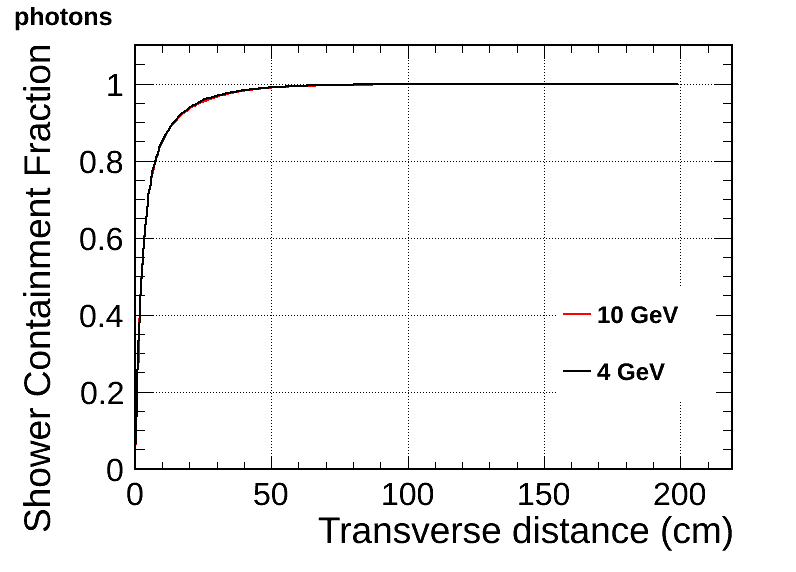
\includegraphics[scale=0.15]{figures/photons_wcont_overlay}\\
%%
%   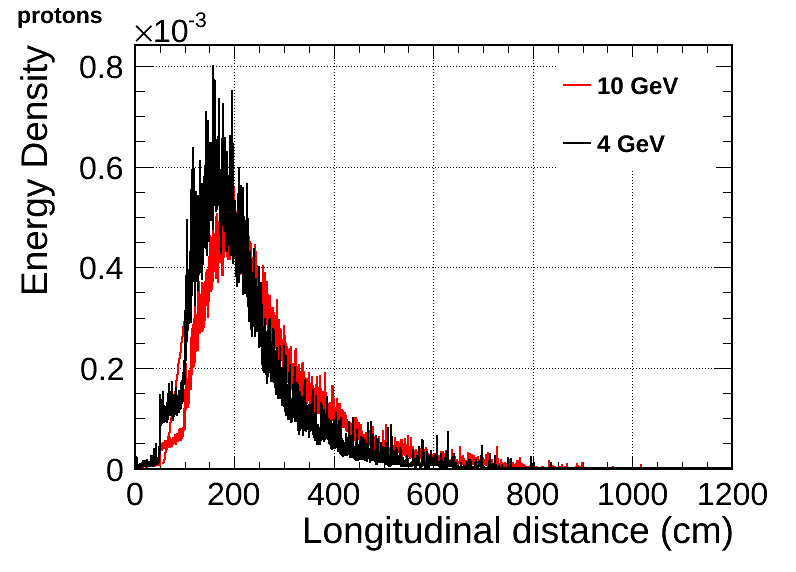
\includegraphics[width=0.31\textwidth,height=3.9cm]{figures/protons_density_overlay}&
   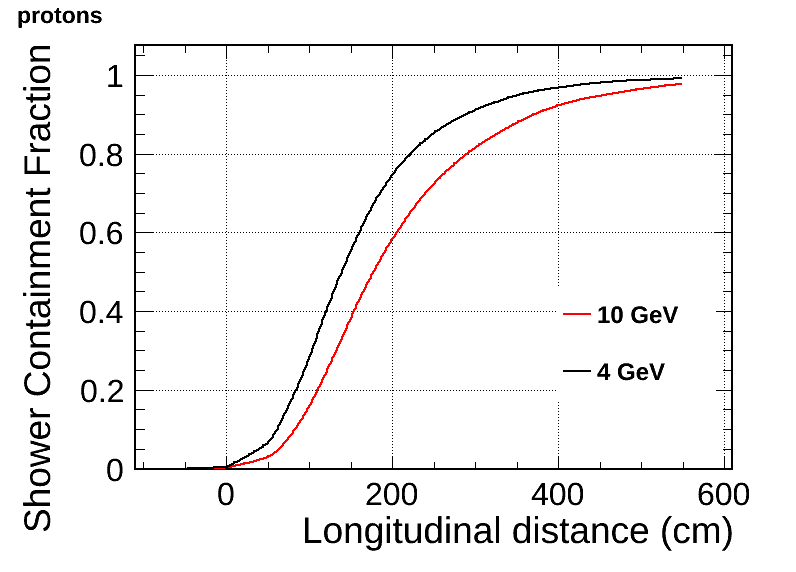
\includegraphics[width=0.49\textwidth,height=4.9cm]{figures/protons_lcont_overlay}&
   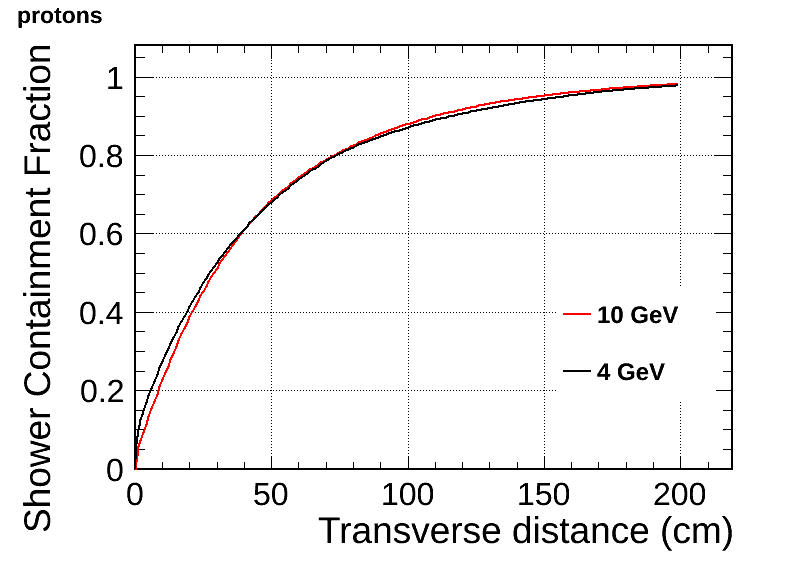
\includegraphics[width=0.49\textwidth,height=4.9cm]{figures/protons_wcont_overlay}\\
%    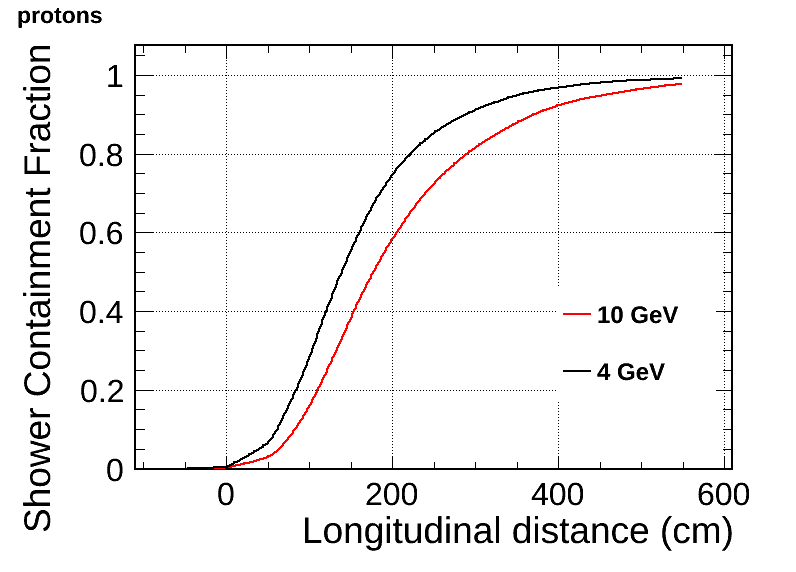
\includegraphics[scale=0.15]{figures/protons_lcont_overlay}&
%    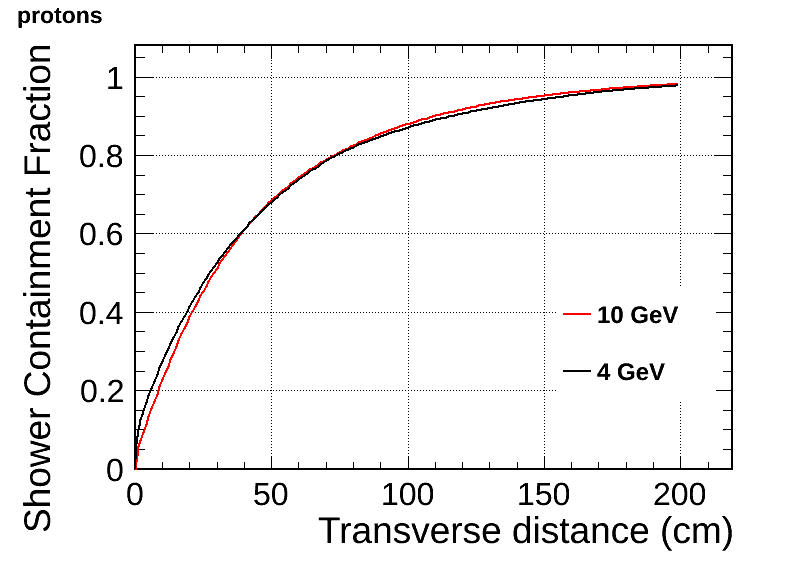
\includegraphics[scale=0.15]{figures/protons_wcont_overlay}\\
% 
%    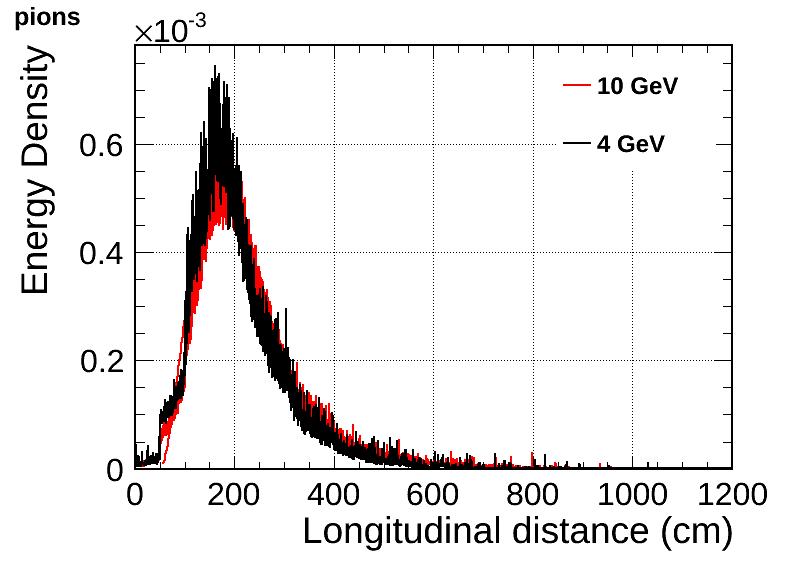
\includegraphics[scale=0.15]{figures/pions_density_overlay}&
%    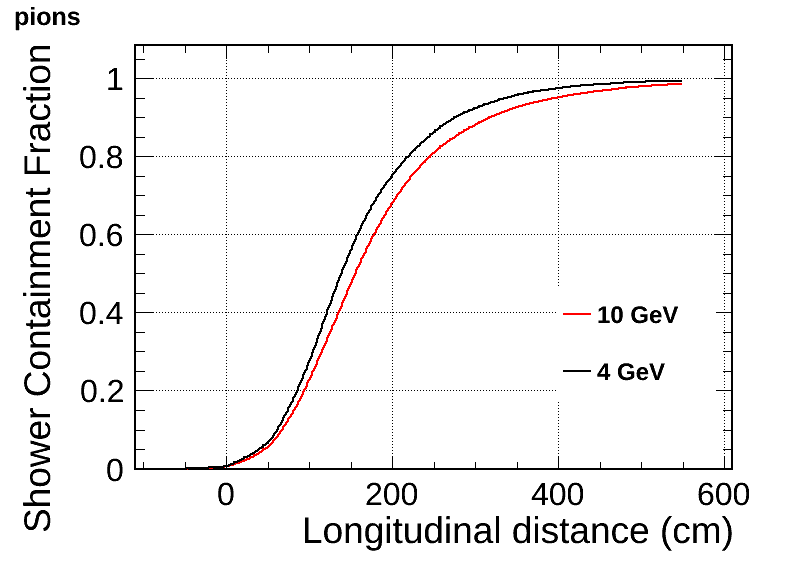
\includegraphics[scale=0.15]{figures/pions_lcont_overlay}&
%    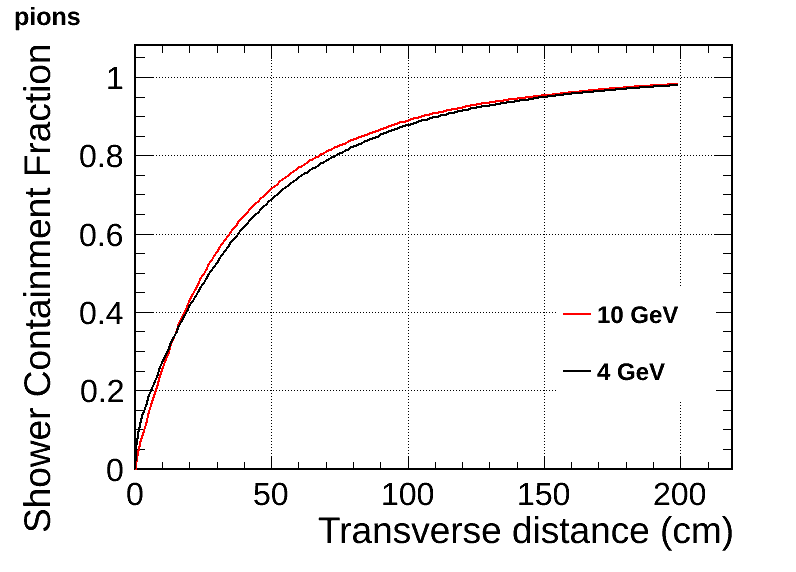
\includegraphics[scale=0.15]{figures/pions_wcont_overlay}\\
 
%   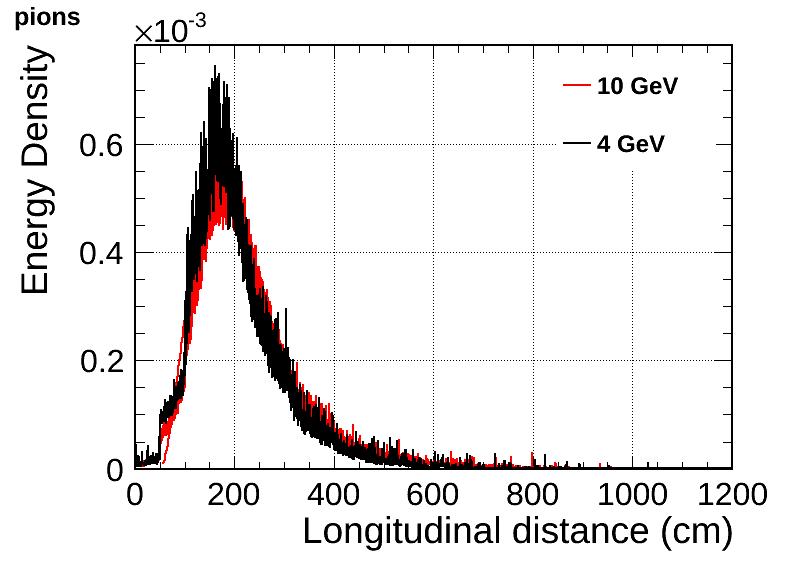
\includegraphics[width=0.31\textwidth,height=3.5cm]{figures/pions_density_overlay}&
%   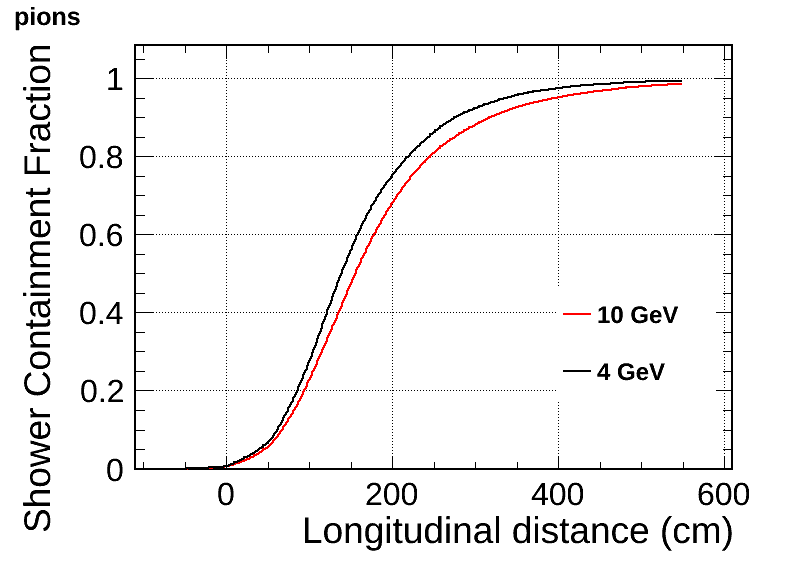
\includegraphics[width=0.31\textwidth,height=3.5cm]{figures/pions_lcont_overlay}&
%   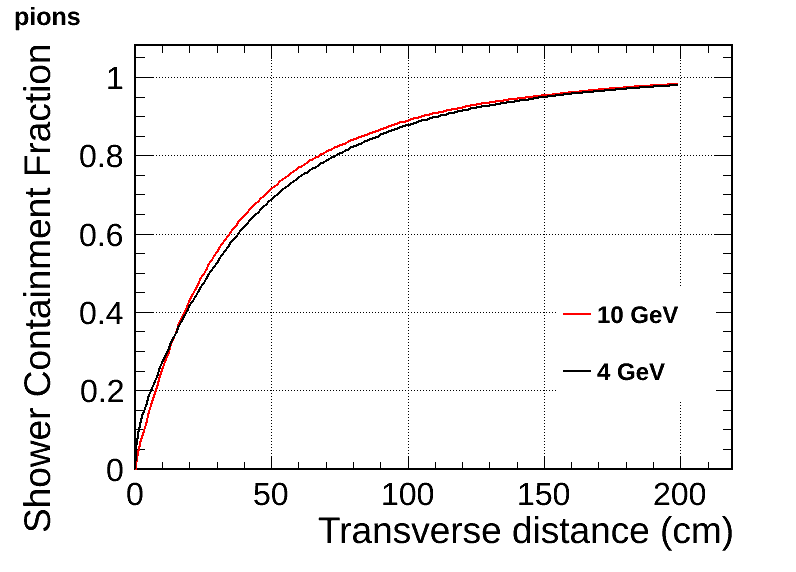
\includegraphics[width=0.31\textwidth,height=3.5cm]{figures/pions_wcont_overlay}\\
%    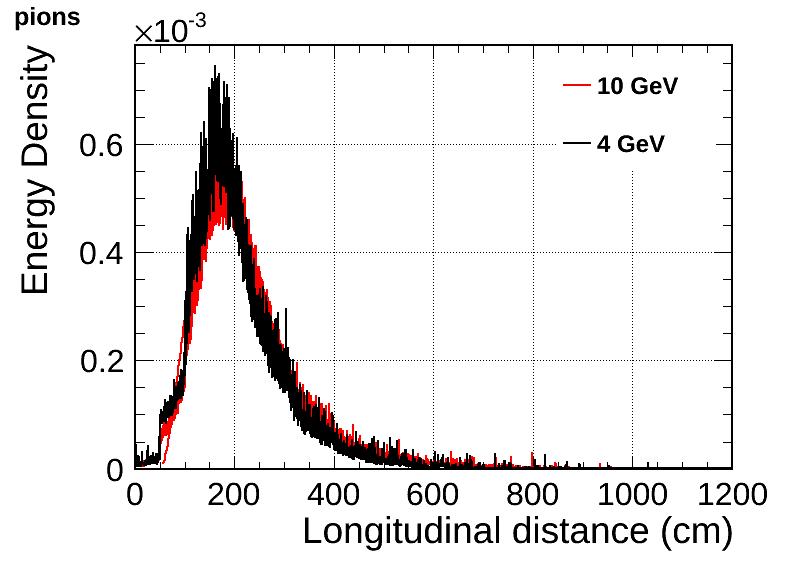
\includegraphics[scale=0.15]{figures/pions_density_overlay}&
%    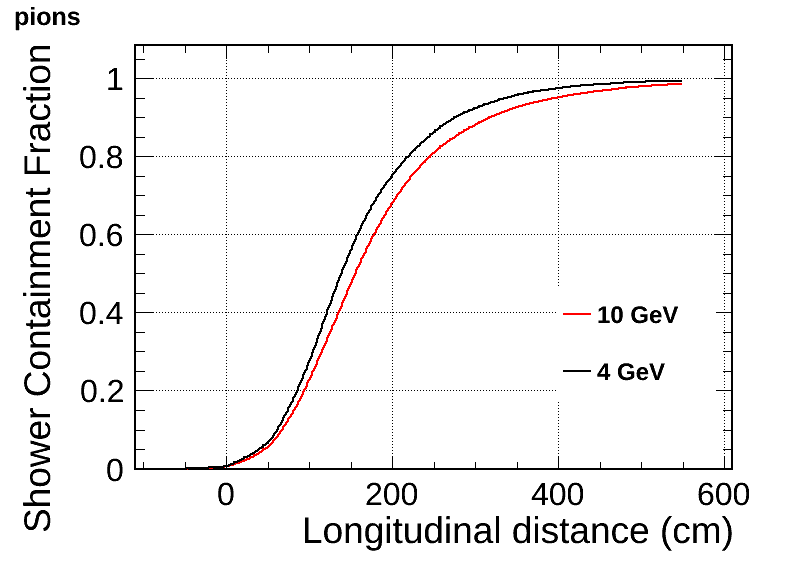
\includegraphics[scale=0.15]{figures/pions_lcont_overlay}&
%    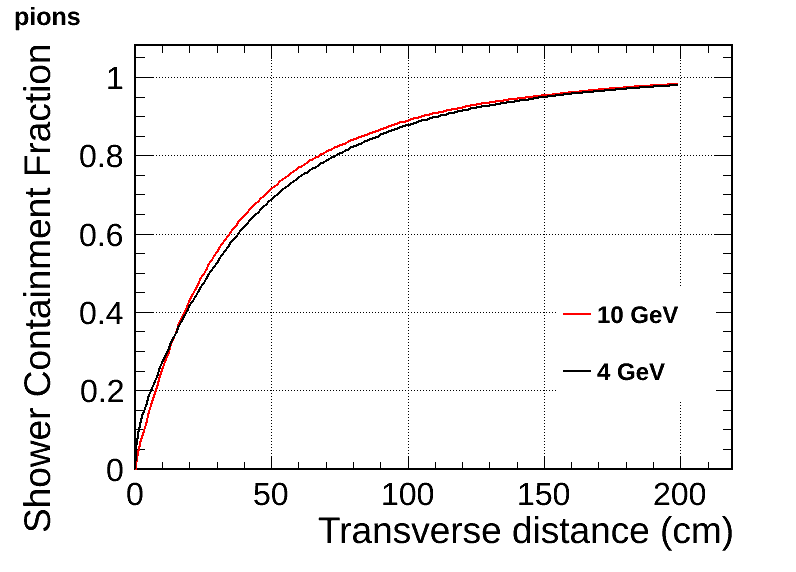
\includegraphics[scale=0.15]{figures/pions_wcont_overlay}\\
 
% 
%    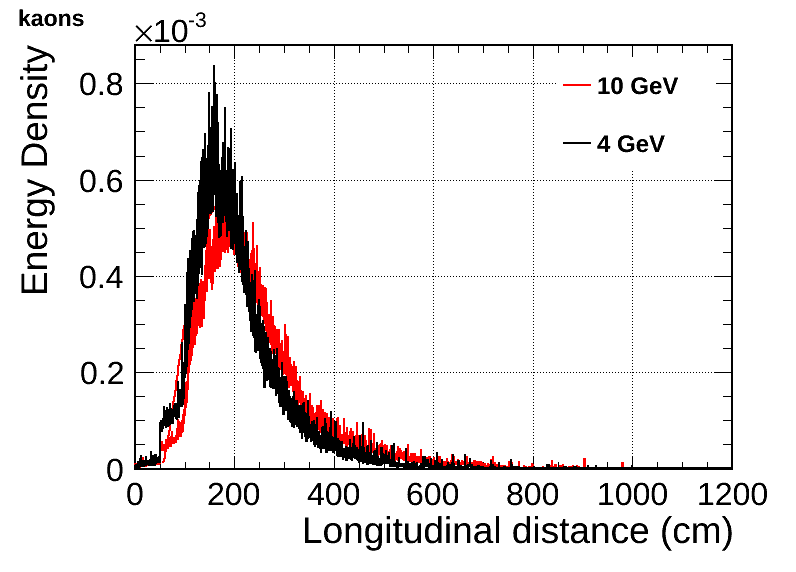
\includegraphics[scale=0.15]{figures/kaons_density_overlay}&
%    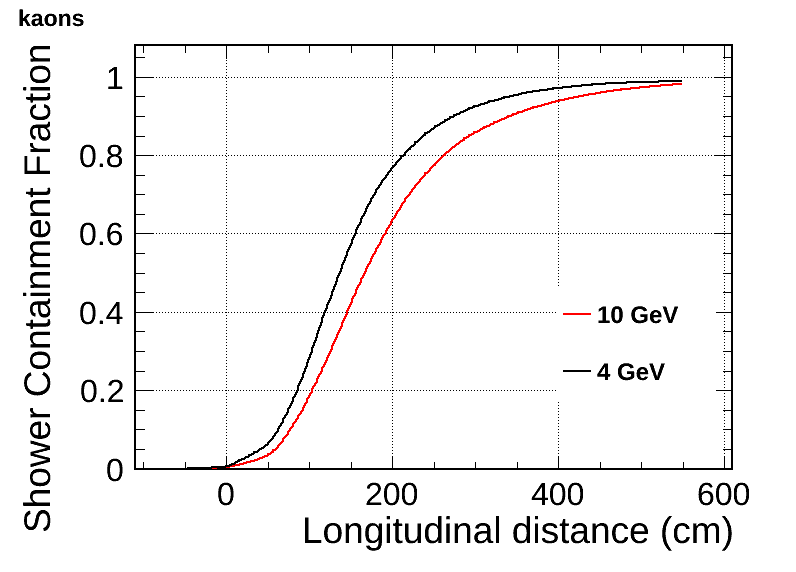
\includegraphics[scale=0.15]{figures/kaons_lcont_overlay}&
%    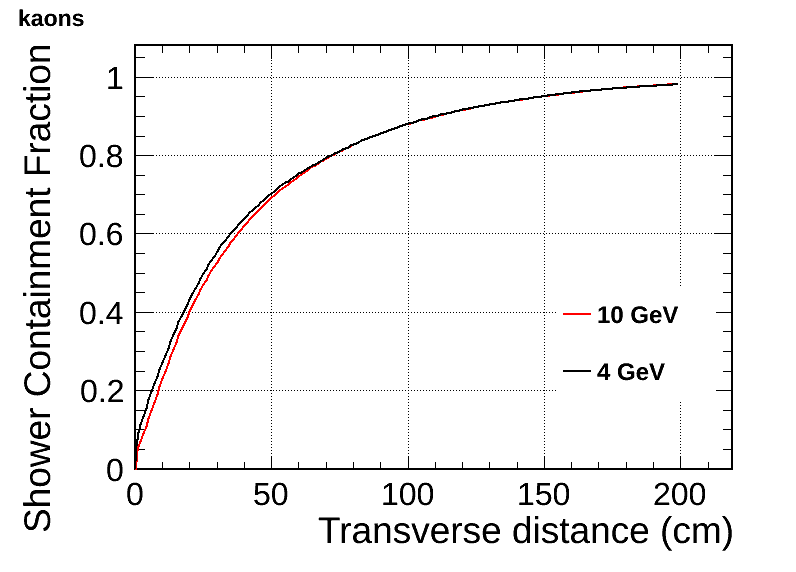
\includegraphics[scale=0.15]{figures/kaons_wcont_overlay}\\
 
  \end{tabular}
  \caption{Simulated longitudinal and transverse containment for proton showers of 4 and 10~GeV/c momenta.
%{\color{red}
%Improve or perhaps remove far left plot (binning too fine).
%Add info on simulation details and containment defn (T. Junk).
%}
}
  \label{fig:containment}  
%For 10 GeV showers, more than 95\% of the energy is contained in a detector of longitudinal size of 550~cm and 
%radius of 200~cm.}
\end{figure}

%\clearpage
%\subsubsection{Particle rates}
%\label{detbeam_rates}
%Estimation of  beam particles rates  necessary to collect high enough statistics in a reasonable time to obtain goals of of the measurements.
% THis should be discussed in the beam section
\subsection {Summary of Beam Particle Requirements}

Table~\ref{tab:runsum} summarizes the requested particle types and momenta along with 
required exposures for the test beam program.
\begin{table}[h]
\centering
\begin{tabular}{|c|c|c|l|}
\hline
Particle & Momenta (GeV/c) & Exposure & Purpose \\ \hline
$\pi^+$       & 0.2, 0.3, 0.4, 0.5, 0.7, 1, 2, 3, 5, 7     &  10K  & hadronic cal, $\pi^0$ content \\ \hline
$\pi^-$       &  0.2, 0.3, 0.4, 0.5, 0.7, 1     &  10K  & hadronic cal, $\pi^0$ content \\ \hline
$\pi^+$   &  2  &  600K & $\pi^o$/$\gamma$ sample \\ \hline
%$\pi^+$ &   1 \& 2  &  10K  & vary angle ($\times$5), reco \\ \hline
proton &  0.7, 1, 2, 3   &  10K & response, PID \\ \hline
proton &  1   &  1M & mis-ID pdk, recombination \\ \hline
e$^+$ or e$^-$       &    0.2, 0.3, 0.4, 0.5, 1, 2, 3, 5, 7        &    10K   & e-$\gamma$ separation/EM shower     \\ \hline
% e$^+$ or e$^-$  &  1 \& 2  &  10K  & vary angle($\times$5), reco \\ \hline
%e$^+$ or e$^-$   (w/rad) &  3  &  20K  & tagged photons \\ \hline
$\mu^-$  &   (0.2), 0.5, 1, 2  &  10K & $E_\mu$, Michel el., charge sign \\ \hline
$\mu^+$ &   (0.2), 0.5, 1, 2   &  10K & $E_\mu$, Michel el.,charge sign  \\ \hline
$\mu^-$ or $\mu^+$ &   3, 5, 7  &  5K & $E_\mu$ MCS \\ \hline
%$\mu^-$ or $\mu^+$  &  1 \& 2  &  5K  & vary angle ($\times$5), reco \\ \hline
%proton &  1 \& 2 &  10K & vary angle ($\times$5), reco \\ \hline
antiproton &  low-energy tune  &  (100) & antiproton stars \\ \hline
K$^+$  & 1 & (13K)   &   response, PID, PDK  \\ \hline
K$^+$  & 0.5, 0.7 & (5K)   &   response, PID, PDK  \\ \hline \hline
$\mu$, e, proton  & 1 (vary angle $\times$5 & 10K  & reconstruction  \\ \hline
\end{tabular}
\caption{Requirements summary for particle types and momenta. Items in parenthesis indicate lower priority (see text).
}
\label{tab:runsum}
\end{table}


Pions and protons spanning the energy range expected in DUNE beam neutrino interactions will be used 
primarily to study hadronic showering reconstruction and calibration as described in Sec.~\ref{sec:showers} as well
as particle identification algorithms discussed in Sec.~\ref{detbeam_pid}). Larger samples of 2~GeV $\pi^+$ and
1 GeV protons will be used to study  secondary $\pi^o$ and protons, respectively, over a large angular range 
to tune and calibration electron/photon separation algorithms (see Sec.~\ref{sec_egam}) and angular
dependent effects on charge collection as described in Sec.~\ref{sec_angle}.
Electrons will be used to benchmark and tune  electron/photon separation algorithms and to calibrate 
electromagnetic showers as discussed in \ref{sec_egam}.
Muon (and antimuon) samples are needed to study reconstruction and PID calibration as well as to obtain 
Michel electron events for calibration  
algorithms for charge-sign determination (see Secs.\ref{sec_reco},\ref{sec_other}).

Charged-kaon samples will be useful to characterize kaon PID efficiency for proton decay sensitivity but
are a somewhat lower priority need. The requested antiproton sample
will be helpful for exotic physics sensitivity studies. Both of these lower priority requests are discussed
in Sec.~\ref{sec_other}.

%Charged pion samples will be used to characterize hadronic shower response and to measure
%absorption cross section parameters on argon.
%for all energies except 0.1 GeV point). 
%Muon samples will be used for calibration and 
%reconstruction tests. Electron samples will be used to measure EM shower response  
%and to tune PID algorithms (statistics shown will far exceed 1\% uncertainty on the mean for 
%EM showers with resolution on the order of 1\% as measured in DOCDB 9434 and 8835. 100k Electron event samples will allow
%high statistics studies of e-gamma separation).  
%Proton response will be studied for reconstruction and to tune PID 
%algorithms. Kaon data will be needed to tune proton decay backgrounds .
%Special runs at various angles with $\pi$, $\mu$, p and electrons will be performed to study reconstruction and tune PID algorithms. 

\subsection{Detector performance tests}

The prototype detector will allow to study the detector response to charge particles from the test beam. The measured energy deposition for various particles and its dependence on the direction of the particle will be used to tune
Monte Carlo simulations and allow more precise reconstruction of neutrino energy and interactions topologies with good particle identification.


\subsubsection{Shower calibration}
\label{sec:showers}

Accurate measurement of neutrino energy will require reconstruction of both electromagnetic and hadronic showers. Reconstruction of hadron energy 
in these energy range will require knowledge of the initiating hadron's 
($\pi^{+/-}$, $p$, or $K^{+/-}$)
fate (interact, decay, or stop). For the case of  interacting hadrons 
the composition of secondaries, which will include neutrals, particles which 
deposit energy electromagnetically ($\pi^o$, $\gamma$), as well as 
secondary hadrons,
%and their energy responses 
will need to be determined to characterize the response. 
The test beam with known incoming particle type and momentum will be used
to characterize interacting hadrons in this energy range.
%quantify responses to initiating hadrons
%($\pi^{+/-}$, $p$, or $K^{+/-}$)
%Hadronic showers initiated by protons in this energy range require

Fig.~\ref{fig:hadronshwr} shows the fraction of true energy deposited by interacting protons with 1~GeV/c (left) and
3~GeV/c (right) incident momenta simulated using FLUKA particle transport code~\cite{fluka05}. 
Interacting protons (65\% of  sample 1~GeV/c) are selected.
% The remaining 
%35\% which range out are be used to study particle identification algorithms (PID) (see Sec.~\ref{detbeam_pid}). 
Reconstruction is performed with ICARUS spatial and calorimetric reconstruction algorithm~\cite{icarus_reco}.
For this study, visible energy is summed using hit information with corrections applied for electron lifetime.
(No attempt is made to correct for electromagnetic shower fractions). 
The resulting energy deposition in the two cases cannot be 
accurately characterized by an average shower calibration factor. Monte Carlo simulations of 
outgoing particles, especially at low energies, must be checked and bench-marked against calibration data to avoid
large uncertainties from shower modeling. 
\begin{figure}[h!]
  \centering
%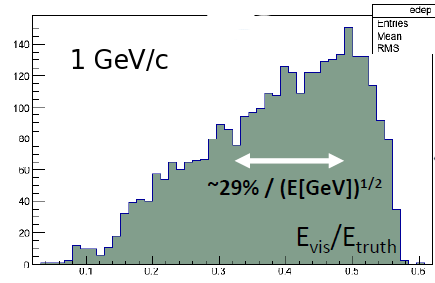
\includegraphics[width=0.49\textwidth,height=5.0cm]{figures/protons_1gev_v0}
%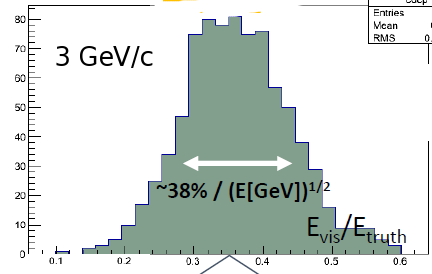
\includegraphics[width=0.49\textwidth,height=5.0cm]{figures/protons_3gev_v0}
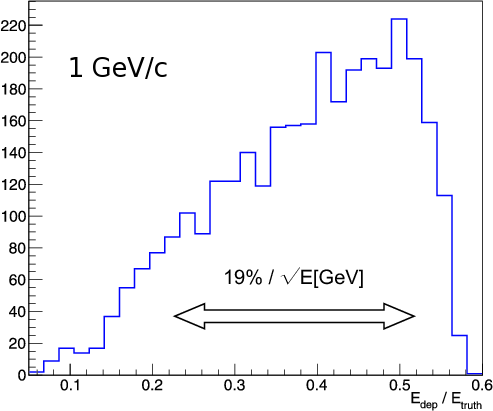
\includegraphics[width=0.49\textwidth,height=5.0cm]{figures/pr1GeV_1}
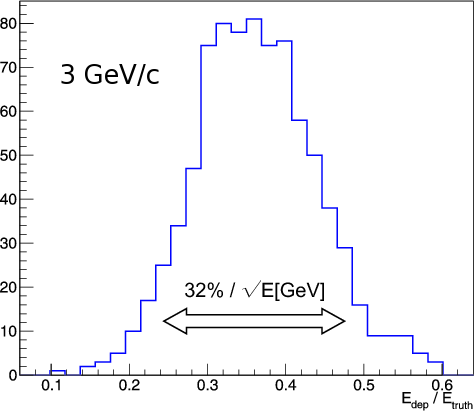
\includegraphics[width=0.49\textwidth,height=5.0cm]{figures/pr3GeV_1}
\label{fig:hadronshwr}
  \caption{Fraction of true energy deposited by interacting protons of 1~GeV/c (left) and
3~GeV/c (right) momenta simulated using FLUKA~\cite{fluka05}.
}
\label{fig:hadronshwr}
\end{figure}

Pion showers at low energies will also be important both for determining the interacted neutrino energy as well
as for modeling neutral current backgrounds resulting from $\pi^o$ content in showers. Differences in energy deposited
by $\pi^+$ versus $\pi^-$ initiated interactions are present up to momenta on the order of 1~GeV/c due to different
final state particles and interaction cross sections. This is illustrated in 
Fig.~\ref{fig:pionshwr} which shows the differences in mean energy deposited (left) and width (right) 
for interacting pions ranging from 0.2~GeV/c up to 5~GeV/c momenta simulated using FLUKA~\cite{fluka05}.
Resulting shower calibrations and reconstruction will differ and therefore each charge must be separately
studies. 
\begin{figure}[h!]
  \centering
%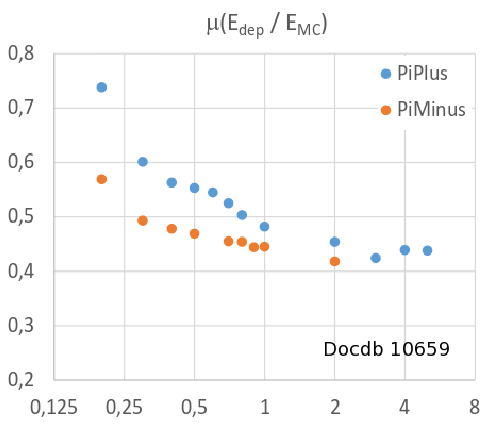
\includegraphics[width=0.49\textwidth,height=5.0cm]{figures/pi+pi-_means}
%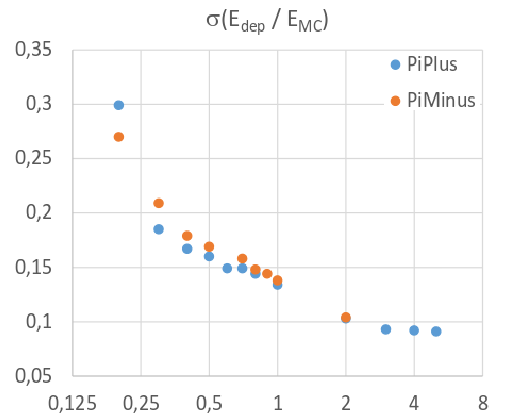
\includegraphics[width=0.49\textwidth,height=5.0cm]{figures/pi+pi-_sig}
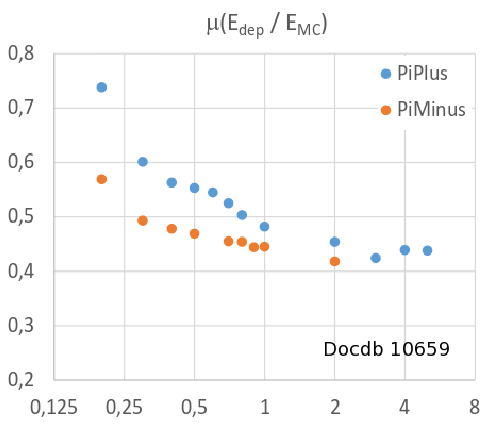
\includegraphics[width=0.49\textwidth,height=5.0cm]{figures/pi+pi-_means}
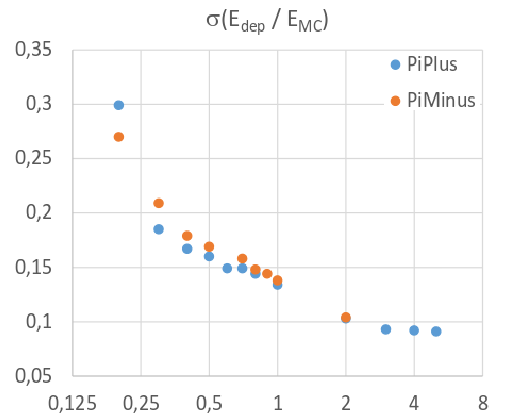
\includegraphics[width=0.49\textwidth,height=5.0cm]{figures/pi+pi-_sig}
  \caption{Differences in mean energy deposited (left) and width of visible energy (right) 
for interacting $\pi^+$ versus $\pi^-$ ranging from 0.2~GeV/c up to 5~GeV/c. 
{\color{red}
Awaiting improved figure
}
}
\label{fig:pionshwr}
\end{figure}


% 
%\begin{table}[h]
%\centering
%\begin{tabular}{|c|c|c|}
%\hline
%Particle     & Momenta (GeV)                                                                                       & Exposure/bin (total)  \\ \hline
%$\pi ^+ $   & 0.2-1.0 (100MeV bins), 1.0-10.0 ( 200MeV bins)    &  1000 (48k)     \\ \hline
%$\pi ^- $    & 0.2-1.0 (100MeV bins), 1.0-10.0 ( 200MeV bins)    &  1000 (48k)     \\ \hline
%$e^+$       & 0.2-10  (100MeV bins), 1.0-10.0 ( 200MeV bins)    &  1000 (48k)       \\ \hline
%$e^- $       & 0.2-10  (100MeV bins), 1.0-10.0 ( 200MeV bins)    &  1000 (48k)       \\ \hline
%$\mu^+$   & 0.2-1.0 (100MeV bins), 1.0-10.0 ( 200MeV bins)    &  1000 (48k)     \\ \hline
%$\mu^-$    & 0.2-1.0 (100MeV bins), 1.0-10.0 ( 200MeV bins)    &  1000 (48k)     \\ \hline
%$p$          &  0.2-1.5 (100MeV bins), 1.5-10.0 ( 200MeV bins)    &  1000 (56k)     \\ \hline
%$\bar p$   &  0.2-1.5 (100MeV bins), 1.5-10.0 ( 200MeV bins)    &  1000 (56k)     \\ \hline
%$K^+$      &  0.2-1.5 (100MeV bins), 1.5-10.0 ( 200MeV bins)    &  1000 (56k)     \\ \hline
%$K^- $      &  0.2-1.5 (100MeV bins), 1.5-10.0 ( 200MeV bins)    &  1000 (56k)     \\ \hline
%\end{tabular}\caption{Data sample requirements for shower calibrations.  Currently about 1k particles is assumed per bin to include variations in the shower topologies. Details MC analysis is necessary. }
%\end{table}
%


\subsubsection{Cross section measurements}


Final state pions are produce copiously in neutrino interactions in this energy range 
and contribute substantially to total visible energy in the interaction.
In neutrino interactions, these particles can reinteract or be absorbed in the nuclear medium
and substantially change the visible energy deposited in the event. 
Therefore, energy dependent cross sections for these processes must be
accurately known to model the effect on reconstructed neutrino energy. 

Current ranges and level of uncertainties.
Precise measurement of the  absorption and charge exchange of pions and kaons. 

Pion absorption is a large part of the pion nucleon cross section from 50 MeV to 500MeV with 
no data above about 1GeV pion kinetic energy. 
%\item pion absorption on argon - Kotlinski, EPJ 9, 537 (2000)
%\item pion cross section as a function of A - Gianelli PRC 61, 054615 (2000)

%There is not currently a satisfactory theory describing absorption. The Valencia group (Vicente-Vacus NPA 568, 855 (1994)) developed model of    the pion-nucleus reaction with fairly good agreement, although not in detail. The actual  mechanism of multi-nucleon absorption
% is not well understood. 
 


\subsubsection{Angular Dependence}

\label{sec_angle}

%Ionization charge deposited by charged-particles in the LAr TPC must be calibrated to
%account for recombination effects. 

A track angular dependent correction must be
%Track angle must be accounted for and a correction
applied to deposited charge to accurately calibrate
dE/dx needed for track momentum and particle ID (see Sec.~\ref{debeam_pid}). 
Charge recombination effects could be angular dependent and
introduce a component that
is currently not modeled. 
For example, Jaffe columnar recombination model~\cite{jaffe,eqref} predicts 
angular dependence given by 
$$Q \approx \frac{Q_o}{1+k_c (dE/dx) / {\cal E} \sin\phi}, $$ 
where
%Recombination modeling 
$Q_o$ and $Q$ are the ionization charge and the collected charge respectively, 
%$dE/dx$ is range based stopping power.
$k_c$ is a constant that depends on LAr diffusion and mobility coefficients, $\cal E$ 
is the electric field strength, and $\phi$ is the angle relative to the drift direction.
%
Simulations performed by ICARUS and LArSoft do no currently incorporate 
an angular dependent effect. (ArgoNeuT~\cite{arogneut_angle} suggests a 
modified Box model with explicit angular dependence can be incorporated 
into Birk's law  by replacing ${\cal E}$  with ${\cal E} \sin\phi$).
Recent results from ArgoNeuT~\cite{argoneut_angle} measure small angular dependent effects using 
stopping protons from neutrino interactions in the range 50-300 MeV with angles from 40-90$^o$.

Test beam data will be used to study angular dependence using 
samples of secondary stopping protons produced in showers at small angles with
respect to the field direction.

\subsubsection{Bethe-Bloch parametrization of charged particles and PID}



%\begin{table}[h]
%\centering
%\begin{tabular}{|c|c|c|}
%\hline
%Particle     & Momenta (GeV)                                                                                       & Exposure/bin (total)  \\ \hline
%$\pi ^+ $   & 0.2-1.0 (50MeV bins), 1.0-3.0 ( 100MeV bins), 3.0-10 ( 200MeV bins)    &  200 (16.6k)     \\ \hline
%$\pi ^- $    & 0.2-1.0 (50MeV bins), 1.0-3.0 ( 100MeV bins), 3.0-10 ( 200MeV bins)    &  200 (16.6k)     \\ \hline
%$e^+$       & 0.2-10  (200MeV bins)                                                                              &  200 (9.8k)        \\ \hline
%$e^- $       & 0.2-10  (200MeV bins)                                                                              &  200 (9.8k)        \\ \hline
%$\mu^+$   & 0.2-1.0 (50MeV bins), 1.0-3.0 ( 100MeV bins), 3.0-10 ( 200MeV bins)    &  200 (16.6k)    \\ \hline
%$\mu^-$    & 0.2-1.0 (50MeV bins), 1.0-3.0 ( 100MeV bins), 3.0-10 ( 200MeV bins)    &  200 (16.6k)     \\ \hline
%$p$          &  0.2-1.5 (50MeV bins), 1.5-3.0 ( 100MeV bins), 3.0-10 ( 200MeV bins)    &  200 (17.2k)     \\ \hline
%$\bar p$   &  0.2-1.5 (50MeV bins), 1.5-3.0 ( 100MeV bins), 3.0-10 ( 200MeV bins)    &  200 (17.2k)    \\ \hline
%$K^+$      &  0.2-1.5 (50MeV bins), 1.5-3.0 ( 100MeV bins), 3.0-10 ( 200MeV bins)    &  200 (17.2k)      \\ \hline
%$K^- $      &  0.2-1.5 (50MeV bins), 1.5-3.0 ( 100MeV bins), 3.0-10 ( 200MeV bins)    &  200 (17.2k)    \\ \hline
%\end{tabular}\caption{Data sample requirements for the $dE/dx$ Bethe-Bloch parametrisation. The lower range starts with the nominal 200 MeV which is not achievable for p and difficult for K. The rough estimate is that we need about 200 particles per bin assuming that about half of them will be actually measured it gives  10\% statistical error for each bin but lower for the fit to the Bethe-Bloch formula. About half of the data sample is in the high momenta region, which can be reduce by decreasing number of particles per bin. }
%\end{table}
%
\label{detbeam_pid}

%The reconstruction of events in the LAr TPC is still a challenge but rapid progress has been achieved in recent years (cite pandora and other reconstruction algorithms). Despite the progress reconstruction algorithms have to rely Monte Carlo predictions which don't simulate liquid argon detectors responses correctly. Reconstruction algorithms will benefit greatly from test beam data particularly from the full scale prototype. The reconstruction algorithms will be trained to correctly reconstruct track, electromagnetic and hadronic showers.
%The data of tracks and showers can be used to create a library of reference events with which to tune algorithms.
%which can be used for matching with he neutrino data, similar to the  LEM (library event matching).

Information on range and charge deposition for stopping charged-particles can be used to 
accurately identify particle type as well as measure kinetic energy. 
Fig.~\ref{fig:resrange}  (left) shows track energy loss per unit length (dE/dx) as a function of residual 
track range for muons, pions, protons and kaons for particles simulated using ICARUS MC (ref).
A neutral-net-based algorithm~\cite{nn_pid,rd_pid}
was used to determine particle probability 
functions for each particle hypothesis. Fig.~\ref{fig:resrange}  shows the result for a cross section of events 
in the residual range bin centerd at 6~cm.
PID algorithm depends on the detector effects, configuration, and geometry and 
reconstruction algorithm. (Fig.~\ref{fig:resrange} uses ICARUS geometry with 3~mm pitch, APA configuration may give significantly
different results, especially for pion/muon separation). 
Plots were made for 3mm pitch, we don't have such simulation for APA configuration, it may differ a bit (which does not change much for proton/kaon, but can be significant for pion/muon).
It is therefore important to test PID on real prototype
detector data in presence of all detector effects.


%The tail is used to calibration the MIP response, the region near the end of the track is used
%to give PID information. (WIP)
%Test beam measurements of stopping particles of each type will be used
%to calibrate the energy deposition functions and to determine particle 
%mis-ID probabilities. 
\begin{figure}[h!]
  \centering
%\includegraphics[width=0.49\textwidth,height=5.0cm]{figures/pid}
%\includegraphics[width=0.49\textwidth,height=5.0cm]{figures/pid_probabilities}
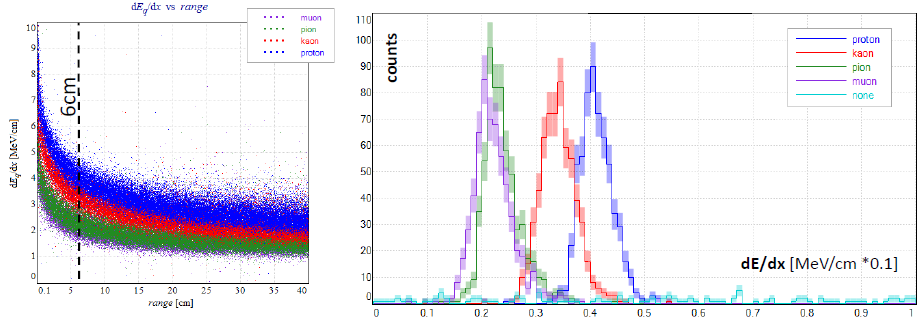
\includegraphics[width=\textwidth,height=5.0cm]{figures/pid_curves}
  \caption{de/dx vs. residual range.
ICARUS geometry with 3~mm pitch is used here, APA configuration may give significantly
different results, especially for pion/muon separation
{\color{red}
Need better versions 
}
}
\label{fig:resrange}
\end{figure}



%collected particle charge, track angle, as well as 
%which depends strongly 

\subsubsection{Reconstruction Effects}
\label{sec_reco}

Reconstruction algorithms use all three signal planes for 3D track and event reconstruction. The quality of reconstruction is affected by the two main factors which can be quantified with test beam data:
\begin{itemize}
\item The complexity of the event topology, that includes the number of objects overlapping in 2D projections and the number of possible object associations between 2D projections. The topology complexity depends on the energy of incident particle. Hadronic showers collected with the test beam can provide data sample to assess the reconstruction algorithm performance and test its dependence on the incident particle energy.
\item Orientation of the reconstructed object w.r.t. the readout wires and electron drift direction:
\begin{itemize}
\item Tracks and cascades in the plane parallel or almost parallel to the signal planes have strongly limited variation of the hit drift time, required for the 3D reconstruction; various reconstruction algorithms can show different performance in the real detector conditions for such inclined objects, especially in the presence of the noise affecting hit time reconstruction.
\item 2D projection of objects aligned with the wires of one of the planes is strongly shortened, which limits the amount of information available to the reconstruction algorithm; the two other signal planes can be used for the spatial reconstruction, however, the validation of the correctness of reconstruction, calculated from the 3D object projected to the third plane, is less efficient.

The most important aspect of this issue is the usage of all planes for the charge measurement. If the reconstructed object is aligned with Collection wires then the calorimetric measurement has to be carried out with the signal of Induction planes. Additional shielding wire plane of the DUNE design will improve the quality of the bipolar signal of Induction planes and the test beam experiment will help with its calibration.
\item Objects aligned with the drift field are projected to a low number of wires and have a large span of drift time. Wire signals of such objects are significantly different than those of objects at higher angles w.r.t. the drift field, requiring a dedicated signal processing for the hit reconstruction. In such orientation also the correction of eventual angular dependence of the recombination effect should be included in the calorimetric reconstruction and calibrated with real data.
\end{itemize}
\end{itemize}

%Main issues for the reconstruction algorithms:
%\begin{itemize}
%\item Reconstruction algorithms use all three signal planes for 3D track and event reconstruction. 
%If the orientation of the track/shower is such that it is aligned with wires on one of the planes, it significantly reduces quality of reconstructed objects. 
%\item Calorimetry with collection and induction planes. In the ICARUS experiment the deposited energy was reconstructed from the signal on the collection plane. The induction planes bipolar signal wasn't "stable" enough to use it for calorimetric measurement. In the ELBNF design there is additional shielding  wire plane which will improve the quality of the bipolar signal and the  test beam experiment will help with its calibration.
%\item   Vertexing.
%\item Reconstruction efficiency for low energy particles. The reconstruction algorithm suffer from the lose of efficiency for low energy particle or particles which leave less than 200-300 hits. Training the algorithms on a low energy particles from the test beam will improve the quality and efficiency of the reconstructed objects.
%\end{itemize}

Any reconstruction algorithm will depend on the particular choices in the TPC design. 
Therefore bench-marking our reconstruction algorithms with a prototype of the final design will
be invaluable to understand the performance of reconstruction.

%
%\begin{table}[h]
%\centering
%\begin{tabular}{|c|c|c|}
%\hline
%Particle     & Momenta (GeV)                                                                                       & Exposure/bin (total)  \\ \hline
%$\pi ^+ $   & 0.2-1.0 (100MeV bins), 1.0-10.0 ( 200MeV bins)    &  500 (26.5k)     \\ \hline
%$\pi ^- $    & 0.2-1.0 (100MeV bins), 1.0-10.0 ( 200MeV bins)    &  500 (26.5k)     \\ \hline
%$e^+$       & 0.2-10  (100MeV bins), 1.0-10.0 ( 200MeV bins)    &  500 (26.5k)       \\ \hline
%$e^- $       & 0.2-10  (100MeV bins), 1.0-10.0 ( 200MeV bins)    &  500 (26.5k)       \\ \hline
%$\mu^+$   & 0.2-1.0 (100MeV bins), 1.0-10.0 ( 200MeV bins)    &  500 (26.5k)     \\ \hline
%$\mu^-$    & 0.2-1.0 (100MeV bins), 1.0-10.0 ( 200MeV bins)    &  500 (26.5k)     \\ \hline
%$p$          &  0.2-1.5 (100MeV bins), 1.5-10.0 ( 200MeV bins)    &  500 (27.8k)     \\ \hline
%$\bar p$   &  0.2-1.5 (100MeV bins), 1.5-10.0 ( 200MeV bins)    &  500 (27.8k)     \\ \hline
%$K^+$      &  0.2-1.5 (100MeV bins), 1.5-10.0 ( 200MeV bins)    &  500 (27.8k)     \\ \hline
%$K^- $      &  0.2-1.5 (100MeV bins), 1.5-10.0 ( 200MeV bins)    &  500 (27.8k)     \\ \hline
%\end{tabular}\caption{Data sample requirements for the development of the reconstruction algorithms. The most important are  the low momenta particles where the showers are more likely to have different topologies. }
%\end{table}


\subsubsection{e/$\gamma$ separation}
\label{sec_egam}

The search for a CP violation phase using $\nu_e$ appearance 
in a $\nu_\mu$ beam requires good electron/photon separation.
Backgrounds originating from photons produced primarily from 
final state $\pi^0$'s must be identified and removed from the signal
electron sample. 


The photons can undergo two process: pair production and Compton scattering. 
The dominant process for photons with energies of several hundreds MeV  is 
the e$^+$ e$^-$ pair production, but Compton scattering also occur at this 
energies. For pair production the e/$\gamma$ separation is achieved by looking 
at the beginning of the electromagnetic shower, where for election we see energy 
deposition typical for single MIP and for photon we see energy deposition consisted 
with two MIPs. In case of Compton scattering off of atomic electrons the 
signal is much more difficult to distinguish from the CC $\nu_e$ scattering signal.


\begin{figure}[h!]
  \centering
%\includegraphics[width=0.49\textwidth,height=5.0cm]{figures/pid}
%\includegraphics[width=0.49\textwidth,height=5.0cm]{figures/pid_probabilities}
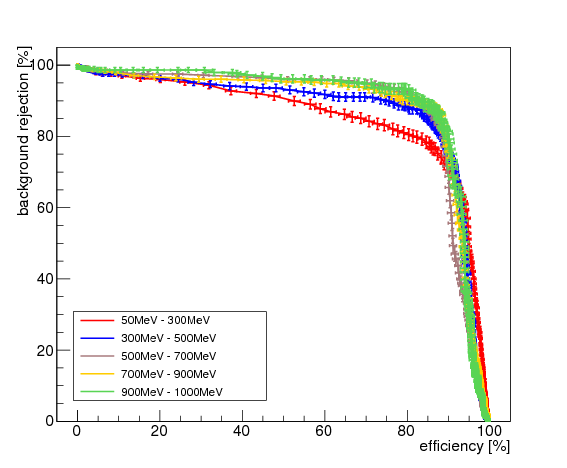
\includegraphics[width=0.49\textwidth,height=6.0cm]{figures/eff-bgdrej-diffen}
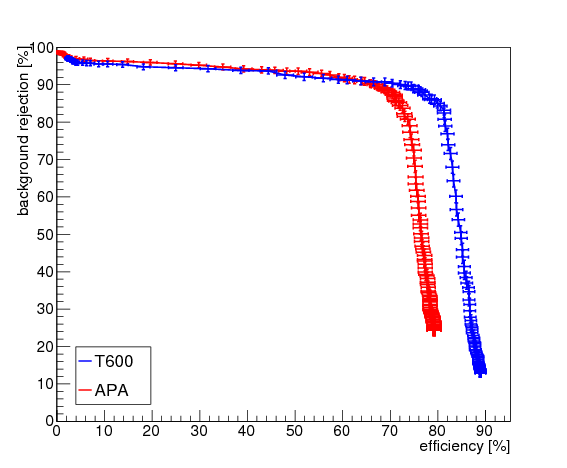
\includegraphics[width=0.49\textwidth,height=6.0cm]{figures/APAT600_all_norm}
\label{fig:egam}
  \caption{(Left)Background rejection versus signal efficiency for various energies.
{\color{red}
}
}
\end{figure}
Electron-photon separation has been studied in LAr TPCs
(ICARUS~\cite{icarus_eg} and ArgoNeuT~\cite{argoneut_eg}).
% numbers come from Dorotas plot docdb 10660 
%as shown in Fig.~\ref{fig:egam1}.
%Currently the 
%separation efficiency is estimated to be at the level of of 95 \% (?) 
Fig.~\ref{fig:egam} shows results of the separation algorithm applied to Monte Carlo event
samples from ??? (more needed in text on the assumptions). 
Background rejection as a function of signal
selection efficiency depends mildly
on incoming particle energies in the range of interest. 
Greater than 90\% background rejection can be 
achieved with $>$70\% efficiency for energies above 300~MeV. (Above 1~GeV 
rejection is even greater at high efficiency).
Our studies indicate that rejection and efficiency depend 
on particular features of the geometry including wire pitch and plane 
orientation which affect the reconstruction. 
Therefore, it is critically important 
to study e/$\gamma$ separation in a prototype LAr TPC detector.

%More discussion of specific samples to be used here.
% move to table section.



\subsection{Other measurements} 
\label{sec_other}

\subsubsection{Supernova and Michel electrons}
The energies of the electrons coming from CC $\nu_e$ interactions from Supernova will be in the order of 10s of MeV. 
The beam test cannot offer such low energy electron, but one can use the Michel electrons form $\mu$ decay to cover these energies. 
 We plan to use the Michel spectrum to calibrate the absolute energy scale. 


%\begin{table}[h]
%\centering
%\begin{tabular}{|c|c|c|}
%\hline
%Particle     & Momenta (GeV/c)    & Exposure/bin  \\ \hline
%$\mu^+$   & (0.2), 0.5, 1      &  10K    \\ \hline
%\end{tabular}\caption{Stopping . }
%\end{table}


\subsubsection{Charge sign determination}
It is not possible to determine the charge of the particle on an event by event basis with non-magnetized LAr TPC detectors. A statistical separation will be studied which will make use of differences in muon versus antimuon capture cross sections and lifetime.
%However, the statistical analyst will be possible. We will fit the muon's half time which is different for muons and antimony due to different muon capture cross sections. 
For the $\mu^+$ for argon we expect about xx\% to be captured and for $\mu^-$ about yy\%. 




\subsubsection{Proton decay sensitivity and background samples}


The DUNE experiment in the deep underground location will seek to detect several modes of proton decay.
In particular, a first ever LAr detector of this scale underground will primarily improve sensitivity to 
proton decays with final state kaons such as  $p \rightarrow K^+ \overline{\nu}$. 
Sensitivity to this process is studied in \cite{bueno}. $K^+$ detector efficiencies are estimated to be $>$97\% in the
appropriate momentum range (500-800 MeV/c). The kaon samples requested in Table~\ref{pdktable} are needed to directly measure 
$K^+$ PID and detection efficiencies. Obtaining low energy kaons will likely be difficult in this beamline.
A sample of 13K beam kaons with 1~GeV/c momentum are requested to provide 2K stopping $K^+$ track samples for PID studies.
(only 15\% of $K^+$ at 1 GeV stop at 1~GeV/c).


%\begin{table}[h]
%\centering
%\begin{tabular}{|c|c|c|}
%\hline
%Particle     & Momenta (GeV/c) & Exposure/bin  \\ \hline
%\hline
%K$^+$  &  1 & (13k)    \\ \hline
%K$^+$  & 0.5, 0.7 & (5k)   \\ \hline
%proton &  1  &  (1M)  \\ \hline
%\end{tabular}\caption{Samples related to proton decay physics requirements.}
%\label{pdktable}
%\end{table}

A sizable sample of protons ($\sim 10^6$)
are requested to study the possible background contributions to  $p \rightarrow K^+ \overline{\nu}$.
This sample of  protons are needed to quantify the possibility that an interacting {\bf p} 
is  {\em mis-IDed as stopping K}. A proton interaction which produces neutrals and one charged pion 
(which is mis-IDed or subsequently decays to $\mu$) can fake the final state kaon signal.


\subsubsection{Anti-proton annihilation }

A sample of antiproton would be useful to calibrate the $p$-$\overline{p}$ annihilation process. 
This would provide input to exotic B-violating process neutron oscillation (reference) modeling of 
subsequent  $n$-$\overline{n}$ annihilation. These events would be tagged in the mixed-mode beam.
Events should be at the lowest energies achievable in this beamline.



